
\chapter{The Central Role of the Propensity Score in Observational Studies for Causal Effects}\label{chapter::pscore-key}
\chaptermark{Propensity Score} 
 
 
\citet{rosenbaum1983central}   proposed the key concept {\it propensity score} and discussed its role in causal inference with observational studies. It is one of the most cited papers in statistics, and \citet{titterington2013biometrika} listed it as the second most cited paper published in {\it Biometrika} during the past 100 years. Its number of citations has grown very fast in recent years. 


Under the IID sampling assumption, we have four random variables associated with each unit: $\{  X, Z, Y(1), Y(0) \} $. Following the basic probability rules, we can factorize the joint distribution as 
\begin{eqnarray*}
&&\pr \{  X, Z, Y(1), Y(0) \}  \\
 &=& \pr(X)  
\times   \pr\{ Y(1), Y(0) \mid X \}   
 \times  \pr\{  Z\mid X, Y(1), Y(0)  \} ,
\end{eqnarray*}
where
\begin{enumerate}
\item
 $\pr(X)$ is the covariate distribution, 
 \item
 $\pr\{ Y(1), Y(0) \mid X \}$ is the outcome distribution conditional on the covariates $X$,
 \item
 $\pr\{  Z\mid X, Y(1), Y(0)  \}$ is the treatment distribution conditional on the covariates $X$, also known as the treatment assignment mechanism. 
\end{enumerate}
Usually, we do not want to model the covariates because they are background information happening before the treatment and outcome. If we want to go beyond the outcome model, then we must focus on the treatment assignment mechanism, which leads to the definition of the propensity score.

\begin{definition}
[propensity score]\label{def::pscore}
Define
$$
e(X, Y(1), Y(0)   ) = \pr\{  Z=1\mid X, Y(1), Y(0)  \}
$$
as the {\it propensity score}. Under strong ignorability, we have
$$
 e(X, Y(1), Y(0)   )  = \pr\{  Z=1\mid X, Y(1), Y(0)  \} = \pr(Z=1 \mid X),
$$
so the propensity score reduces to 
$$
e(X) = \pr(Z=1 \mid X),
$$
the conditional probability of receiving the treatment given the observed covariates.  
\end{definition} 

 
\citet{rosenbaum1983central} used  $e(X) = \pr(Z=1 \mid X)$ as the definition of the propensity score because they focused on observational studies under strong ignorability. It is sometimes helpful to view $e(X, Y(1), Y(0)   ) = \pr\{  Z=1\mid X, Y(1), Y(0)  \}$ as the general definition of the propensity score even when strong ignorability fails.  See Problem \ref{hw::principal-unobserved-cov} for more details. 

Following \citet{rosenbaum1983central}, this chapter will demonstrate that $e(X)$ is a key quantity in causal inference with observational studies under ignorability.

 


\section{The propensity score as a dimension reduction tool}

\subsection{Theory}

\begin{theorem}
\label{thm::pscore-dimreduction}
If $Z\ind \{ Y(1), Y(0)  \} \mid X$, then
$
Z\ind \{ Y(1), Y(0)  \} \mid e(X).
$
\end{theorem}

Theorem \ref{thm::pscore-dimreduction} states that if strong ignorability holds conditional on covariates $X$, then it also holds conditional on the scalar propensity score $e(X)$. 
The ignorability requires conditioning on many background characteristics $X$ of the units, but Theorem \ref{thm::pscore-dimreduction} implies that conditioning on the propensity score $e(X)$ removes all confounding induced by covariates $X.$ The original covariates $X$ can be general and have many dimensions, but the propensity score $e(X)$ is a one-dimensional scalar variable bounded between $0$ and $1$. Therefore, the propensity score reduces the dimension of the original covariates but still maintains the ignorability. As a statistical terminology, we can view the propensity score as a {\it dimensional reduction} tool. We will first prove Theorem \ref{thm::pscore-dimreduction}  below and then give an application of the dimension reduction property of the propensity score. 





\begin{myproof}{Theorem}{\ref{thm::pscore-dimreduction}}
By the definition of conditional independence, we need to show that 
\begin{eqnarray}
\pr\{ Z=1\mid Y(1), Y(0), e(X)  \} = \pr\{ Z=1\mid e(X)  \} .
\label{eq::pscore-dimreduction}
\end{eqnarray}
The left-hand side of \eqref{eq::pscore-dimreduction} equals
\begin{eqnarray*}
&&\pr\{ Z=1\mid Y(1), Y(0), e(X)  \}  \\
&=& E\{ Z \mid Y(1), Y(0), e(X)  \}  \\
&=& E\Big[   E\{ Z \mid Y(1), Y(0), e(X) , X  \}  \mid   Y(1), Y(0), e(X)    \Big]  \\
&&\quad  \quad  \quad  \quad   \quad \quad \text{(tower property; see Section \ref{appendix::tower-property})} \\
&=& E\Big[   E\{ Z \mid Y(1), Y(0),   X  \}  \mid   Y(1), Y(0), e(X)    \Big]  \\
&=& E\Big\{    E(Z \mid  X  )  \mid   Y(1), Y(0), e(X)    \Big\}  \quad \text{(strong ignorability)} \\
&=& E\Big\{   e(X) \mid   Y(1), Y(0), e(X)    \Big\} \\
&=& e(X).
\end{eqnarray*}
The right-hand side of \eqref{eq::pscore-dimreduction} equals 
\begin{eqnarray*}
&& \pr\{ Z=1\mid e(X)  \} \\
  &=&  E\{ Z \mid e(X)  \} \\
 &=& E\Big[   E\{ Z \mid e(X), X  \}  \mid e(X)  \Big ] \quad \text{(tower property)} \\
 &=& E\Big\{    E( Z \mid  X )  \mid e(X)  \Big \}   \\
 &=& E\Big\{   e(X)  \mid e(X)  \Big \} \\
 &=& e(X). 
\end{eqnarray*}
So the left-hand side of \eqref{eq::pscore-dimreduction} equals the right-hand side of \eqref{eq::pscore-dimreduction}. 
\end{myproof}


\subsection{Propensity score stratification}
\label{sec::pscore-stratification}




Theorem \ref{thm::pscore-dimreduction} motivates a simple method for estimating causal effects: propensity score stratification. 
Starting from the simple case, we assume that the propensity score is known and only takes $K$ possible values $\{ e_1,\ldots, e_K \}$ with $K$ being much smaller than the sample size $n$. Theorem \ref{thm::pscore-dimreduction} reduces to
$$
Z\ind \{ Y(1), Y(0)  \} \mid e(X) = e_k  \quad (k=1,\ldots, K).
$$
Therefore, we have an SRE, that is, we have $K$ independent CREs within strata of the propensity score. We can analyze the observational data in the same way as the SRE stratified on $e(X)$. 


In general, the propensity score is not known and is not discrete. We often fit a statistical model for $\pr(Z = 1\mid X)$ (for example, a logistic model of the binary $Z$ given $X$) to obtain the estimated propensity score $\hat{e}(X)$. This estimated propensity score can take as many values as the sample size, but we can discretize it to approximate the simple case above. For example, we can discretize the estimated propensity score by its $K$ quantiles to obtain $\hat{e}'(X)$:
$
\hat{e}'(X_i) = e_k,
$
the $k/K$-th quantile of $\hat{e}(X)$,
if $ \hat{e}(X_i)$ is between the $(k-1)/K$-th and $k/K$-th quantiles of the $\hat{e}(X_i)$'s. Then  
$$
Z\ind \{ Y(1), Y(0)  \} \mid \hat{e}'(X) = e_k  \quad (k=1,\ldots, K).
$$
holds approximately. So we can analyze the observational data in the same way as the SRE stratified on $\hat{e}'(X)$. 
The ignorability holds only approximately given $\hat{e}'(X)$. We can further use regression adjustment based on covariates to remove bias and improve efficiency. To be more specific, we can obtain \citet{lin2013}'s  estimator within each stratum and construct the final estimator by a weighted average (see Chapter \ref{sec::covariate-SRE}). 


 




With an unknown propensity score, we need to fit a statistical model to obtain the estimated propensity score $\hat{e}(X)$. This makes the final estimator dependent on the model specification. However, the propensity score stratification estimator only requires the correct ordering of the estimated propensity scores rather than their exact values, which makes it relatively robust compared with other methods. This robustness property of propensity score stratification appeared in many numerical examples but its rigorous quantification is still missing in the literature. 




An important practical question is how to choose $K$? If $K$ is too small, then ignorability does not hold conditional on $\hat{e}'(X)$ even approximately. If $K$ is too large, then we do not have enough units within each stratum of the estimated propensity score and many strata have only treated or control units. Therefore, we face a trade-off. Following \citet{cochran1968effectiveness}'s heuristics, \citet{rosenbaum1983central} and \citet{rosenbaum1984reducing} suggested $K=5$ which removes a large amount of bias in many settings. However, with extremely large datasets, propensity score stratification leads to biased estimators with a fixed $K$ \citep{lunceford2004stratification}. It is thus reasonable to increase $K$ as long as each stratum still has enough treated and control units. \citet{wang2020robust} suggested a greedy choice of $K$, which is the maximum number of strata such that the stratified estimator is well-defined. However, the rigorous theory for this procedure is not fully established. 




Another important practical question is how to compute the standard errors of the estimators based on propensity score stratification. Some researchers have conditioned on the discretized propensity scores $\hat{e}'(X)$ and reported standard errors based on the SRE. This effectively ignores the uncertainty in the estimated propensity scores. This often leads to an overestimation of the true variance since a surprising result in the literature is that using the estimated propensity scores decreases the asymptotic variance for estimating the average causal effect \citep{su2023estimated}. 
Other researchers bootstrapped the whole procedure to account for full uncertainty. However, the theory for the bootstrap is still unclear due to the discreteness of this estimator. 
 
 
 
 \subsection{Application}\label{sec::application-pscore-stratification}


To illustrate the propensity score stratification method, I revisited Example \ref{eg::chan-bmi-ATE}. 
\begin{lstlisting}
> nhanes_bmi = read.csv("nhanes_bmi.csv")[, -1]
> z = nhanes_bmi$School_meal
> y = nhanes_bmi$BMI
> x = as.matrix(nhanes_bmi[, -c(1, 2)])
> x = scale(x)
\end{lstlisting}
Example \ref{eg::chan-bmi-ATE} introduced the covariates in the dataset. The treatment \ri{School_meal} is the indicator for participation in the school meal plan, and the outcome \ri{BMI} is the BMI. 



\begin{figure}
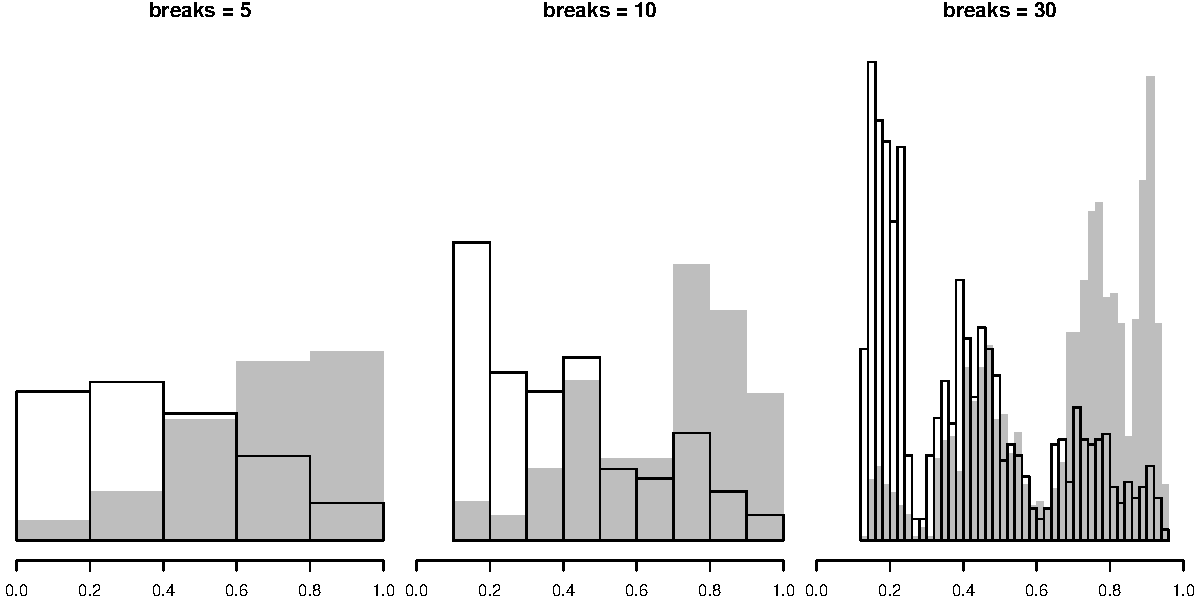
\includegraphics[width = \textwidth]{figures/pscore_stratified_hist.pdf}
\caption{Histograms of the estimated propensity scores based on the \ri{nhanes_bmi} data: white for the control group and grey for the treatment group}\label{fig::pscore_bmi}
\end{figure}


Figure \ref{fig::pscore_bmi} shows the histograms of the estimated propensity scores with different numbers of bins $(K=5,10,30)$. 
Based on propensity score stratification, we can calculate the point estimators and the standard errors for difference choice of $K \in \{5, 10, 20, 50, 80 \}$ as follows (with the function \ri{Neyman_SRE} defined in Chapter \ref{chapter::stratification-poststratification} for analyzing the SRE):
\begin{lstlisting}
> pscore = glm(z ~ x, family = binomial)$fitted.values
> n.strata = c(5, 10, 20, 50, 80)
> strat.res = sapply(n.strata, FUN = function(nn){
+   q.pscore = quantile(pscore, (1:(nn-1))/nn)
+   ps.strata = cut(pscore, breaks = c(0,q.pscore,1), 
+                   labels = 1:nn)
+   Neyman_SRE(z, y, ps.strata)})
> 
> rownames(strat.res) = c("est", "se")
> colnames(strat.res) = n.strata
> round(strat.res, 3)
         5     10     20     50     80
est -0.116 -0.178 -0.200 -0.265 -0.204
se   0.283  0.282  0.279  0.272     NA
\end{lstlisting}
Increasing $K$ from $5$ to $50$ reduces the standard error. However, we cannot go as extreme as $K=80$ because the standard error is not well-defined in some strata with only one treated or one control unit. The above estimators show a negative but insignificant effect of the meal program on  BMI. 


We can also compare the above estimator with the three simple regression estimators: the one without adjusting for any covariates, and Fisher's and Lin's estimators. 
\begin{lstlisting}
> DiM = lm(y ~ z)
> Fisher = lm(y ~ z + x)
> Lin = lm(y ~ z + x + z*x)
> res.regression = c(coef(DiM)[2], hccm(DiM)[2, 2]^0.5,
+                    coef(Fisher)[2], hccm(Fisher)[2, 2]^0.5,
+                    coef(Lin)[2], hccm(Lin)[2, 2]^0.5)
> res.regression = matrix(res.regression,
+                         nrow = 2, ncol = 3)
> rownames(res.regression) = c("est", "se")
> colnames(res.regression) = c("naive", "fisher", "lin")
> round(res.regression, 3)   
    naive fisher    lin
est 0.534  0.061 -0.017
se  0.225  0.227  0.226
\end{lstlisting} 
The naive difference in means differs greatly from the other methods due to the large imbalance in covariates. Fisher's estimator still gives a positive point estimate although it is not significant. Lin's estimator and the propensity score stratification estimators give qualitatively the same results. The propensity score stratification estimators are stable across different choices of $K$. 




\section{Propensity score weighting}

\subsection{Theory}

\begin{theorem}
\label{thm::pscore-weighting}
If $Z\ind \{ Y(1), Y(0)  \} \mid X$ and $0<e(X)<1$, then
$$
E\{  Y(1) \} =  E\left\{  \frac{ZY}{e(X)}  \right\},\quad
E\{  Y(0) \} =  E\left\{  \frac{(1-Z)Y}{1-e(X)}  \right\} ,
$$
and
$$
\tau = E\{  Y(1) -  Y(0) \} =  E\left\{  \frac{ZY}{e(X)} - \frac{(1-Z)Y}{1-e(X)}   \right\} .
$$
\end{theorem}


Before proving Theorem \ref{thm::pscore-weighting}, it is important to note the additional assumption $0<e(X)<1$. It is called the {\it overlap} or {\it positivity} condition. The formulas in Theorem \ref{thm::pscore-weighting} become infinity if $e(X)=0$ or $1$ for some values of $X$. It is not a requirement only for the identification formulas based on propensity score weighting. Although it was not stated explicitly in Theorem \ref{thm::identification-formula}, the conditional expectations $E(Y\mid Z=1, X)$ and $ E(Y\mid Z=0, X)$ in the identification formula of $\tau$ in \eqref{eq::nonparametric-identification-tau} is well defined only if $0< e(X) < 1$. The overlap condition can be viewed as a technical condition to ensure that the formulas in Theorems \ref{thm::identification-formula} and \ref{thm::pscore-weighting} are well defined. It can also cause some philosophical issues for causal inference with observational studies. When unit $i$ has $e(X_i)=1$, we always observe its potential outcome under the treatment, $Y_i(1)$, but can never observe its potential outcome under the control, $Y_i(0)$. In this case, the potential outcome $Y_i(0)$ may not even be well defined, making the definition of the causal effect ambiguous for unit $i$. \citet{king2006dangers} called $Y_i(0)$ an {\it extreme counterfactual} when $e(X_i)=1$, and discussed their dangers in causal inference. A similar problem arises if unit $i$ has $e(X_i)=0$. 
 
 
In sum,  $Z\ind \{ Y(1), Y(0)  \} \mid X$ requires adequate covariates to ensure the conditional independence of the treatment and potential outcomes, and $0<e(X)<1$ requires residual randomness in the treatment conditional on the covariates. In fact, \citet{rosenbaum1983central}'s definition of strong ignorability includes both of these conditions. In modern literature, they are often stated separately. 
 


 

\begin{myproof}{Theorem}{\ref{thm::pscore-weighting}}
I only prove the result for $E\{ Y(1) \}$ because the proof of the result for $E\{ Y(0) \}$ is similar. We have
\begin{eqnarray*}
&&E\left\{  \frac{ZY}{e(X)}  \right\} \\
&=& E\left\{  \frac{ZY(1)}{e(X)}  \right\} \\
&=& E\left[ E\left\{  \frac{ZY(1)}{e(X)}  \mid X \right\}  \right]  \quad \text{(tower property)} \\
&=& E\left[  \frac{1}{e(X)}   E\left\{   ZY(1)  \mid X \right\}  \right]   \\
&=& E\left[  \frac{1}{e(X)}   E( Z  \mid X ) E\left\{   Y(1)  \mid X \right\}  \right]  \quad \text{(strong ignorability)} \\\\
&=& E\left[  \frac{1}{e(X)}   e(X) E\left\{   Y(1)  \mid X \right\}  \right] \\
&=& E\left[ E\left\{   Y(1)  \mid X \right\}  \right] \\
&=& E\{   Y(1) \}. 
\end{eqnarray*}
\end{myproof}



\subsection{Inverse propensity score weighting estimators}\label{sec::ipw-estimators}

Theorem \ref{thm::pscore-weighting} motivates the following moment estimator for the average causal effect:
$$
\hat{\tau}^\textup{ht} = \frac{1}{n} \sumn \frac{Z_i Y_i}{ \hat{e}(X_i) }
- \frac{1}{n} \sumn \frac{ (1-Z_i) Y_i}{ 1 - \hat{e}(X_i) } ,
$$
where $\hat{e}(X_i)$ is the estimated propensity score. This is the inverse propensity score weighting (IPW) estimator, which is also called the Horvitz--Thompson (HT) estimator. \citet{horvitz1952generalization} proposed it in survey sampling and \citet{rosenbaum1987model} used in causal inference with observational studies. 


However, the estimator $\hat{\tau}^\textup{ht}$ has many problems. In particular, it is not invariant to the location transformation of the outcome. 
Proposition \ref{prop::no-invariance-HT} states this problem precisely, with the proof relegated to Problem \ref{hw::hajek-weights}. 

\begin{proposition}
[lack of invariance for the HT estimator]
\label{prop::no-invariance-HT}
If we change $Y_i$ to $Y_i+c$ with a constant $c$, then the HT estimator $\hat{\tau}^\textup{ht}$ becomes $\hat{\tau}^\textup{ht} + c (\hat{ 1 }_\textsc{T} - \hat{ 1 }_\textsc{C})$, where 
$$
\hat{ 1 }_\textsc{T}=   \frac{1}{n} \sumn \frac{Z_i }{ \hat{e}(X_i) } ,\quad
\hat{ 1 }_\textsc{C} =\frac{1}{n} \sumn \frac{ (1-Z_i) }{ 1 - \hat{e}(X_i) }   
$$
can be viewed as two different estimates of the constant $1$. 
\end{proposition}

In Proposition \ref{prop::no-invariance-HT}, I use the funny notation $\hat{ 1 }_\textsc{T} $ and $ \hat{ 1 }_\textsc{C}$ because with the true propensity score these two terms both have expectation 1; see Problem \ref{hw::hajek-weights} for more details. 
In general, $\hat{ 1 }_\textsc{T} - \hat{ 1 }_\textsc{C}$ is not zero in finite samples. 
Since adding a constant to every outcome should not change the average causal effect, the HT estimator is not reasonable because of its dependence on $c.$ A simple fix to the problem is to normalize the weights by $\hat{ 1 }_\textsc{T}  $ and $\hat{ 1 }_\textsc{C} $ respectively, resulting in the following estimator 
$$
\hat{\tau}^\textup{hajek} = \frac{  \sumn \frac{Z_i Y_i}{ \hat{e}(X_i) }  }{  \sumn \frac{Z_i }{ \hat{e}(X_i) } }
- \frac{  \sumn \frac{ (1-Z_i) Y_i}{ 1 - \hat{e}(X_i) }  }{  \sumn \frac{ 1-Z_i}{ 1 - \hat{e}(X_i) }  }.
$$
This is the Hajek estimator due to \citet{hajek1971comment} in the context of survey sampling with varying probabilities. We can verify that the Hajek estimator is invariant to the location transformation. That is, if we replace $Y_i$ by $Y_i + c$, then $\hat{\tau}^\textup{hajek}$ remains the same; see Problem \ref{hw::hajek-weights}. Moreover, many numerical studies have found that $\hat{\tau}^\textup{hajek}$ is much more stable than $\hat{\tau}^\textup{ht}$ in finite samples. 





\subsection{A problem of IPW and a fundamental problem of causal inference}
\label{sec::ipw-problem}


Many asymptotic analyses require a {\it strong overlap} condition
$$
0<  \alpha_\textsc{L} \leq e(X) \leq  \alpha_\textsc{U} < 1,
$$
that is, the true propensity score is bounded away from $0$ and $1$. However, \citet{d2017overlap} pointed out that this is a rather strong assumption, especially with many covariates. Chapter \ref{chapter::overlap} will discuss this problem in detail. 


Even if the strong overlap condition holds for the true propensity score, the estimated propensity scores can be close to $0$ or $1$. 
When this happens, the weighting estimators blow up to infinity, which results in extremely unstable behavior in finite samples. We can either truncate the estimated propensity score by changing it to
$$
 \max\Big[  \alpha_\textsc{L},   \min\{   \hat{e}(X_i), \alpha_\textsc{U} \}   \Big] ,
$$
or trim the observations by dropping units with $\hat{e}(X_i)$ outside the interval $[\alpha_\textsc{L},   \alpha_\textsc{U}  ]$. \citet{crump2009dealing} suggested $  \alpha_\textsc{L} = 0.1$ and $\alpha_\textsc{U} = 0.9 $, and \citet{kurth2005results} suggested $  \alpha_\textsc{L} = 0.05$ and $\alpha_\textsc{U} = 0.95 $. \citet{yang2018asymptotic} established some asymptotic theory for trimming. Overall, although trimming often stabilizes the IPW estimators, it also injects additional arbitrariness into the procedure. 




 \subsection{Application}\label{sec::application-pscore-weighting}


The following functions can compute the IPW estimators and their bootstrap standard errors. 
\begin{lstlisting}
ipw.est = function(z, y, x, truncps = c(0, 1))
{
  ## fitted propensity score
  pscore   = glm(z ~ x, family = binomial)$fitted.values
  pscore   = pmax(truncps[1], pmin(truncps[2], pscore))
  
  ace.ipw0 = mean(z*y/pscore - (1 - z)*y/(1 - pscore))
  ace.ipw  = mean(z*y/pscore)/mean(z/pscore) - 
    mean((1 - z)*y/(1 - pscore))/mean((1 - z)/(1 - pscore))
  
  return(c(ace.ipw0, ace.ipw))     
}


ipw.boot = function(z, y, x, n.boot = 500, truncps = c(0, 1))
{
  point.est  = ipw.est(z, y, x, truncps)
  
  ## nonparametric bootstrap
  n.sample   = length(z)
  x          = as.matrix(x)
  boot.est   = replicate(n.boot, {
    id.boot = sample(1:n.sample, n.sample, replace = TRUE)
    ipw.est(z[id.boot], y[id.boot], x[id.boot, ], truncps)
  })
  boot.se    = apply(boot.est, 1, sd)
  
  res = cbind(point.est, boot.se)
  colnames(res) = c("est", "se")
  rownames(res) = c("HT", "Hajek")
  
  return(res)
}
\end{lstlisting}

Revisiting Example \ref{eg::chan-bmi-ATE}, we can obtain the IPW estimators based on different truncations of the estimated propensity scores. The following results are the two weighting estimators with the bootstrap standard errors, with truncations at $(0,1)$, $(0.01, 0.99)$, $(0.05, 0.95)$, and $(0.1, 0.9)$:
\begin{lstlisting}
> trunc.list = list(trunc0 = c(0,1), 
+                   trunc.01 = c(0.01, 0.99), 
+                   trunc.05 = c(0.05, 0.95), 
+                   trunc.1 = c(0.1, 0.9))
> trunc.est = lapply(trunc.list,
+                    function(t){
+                      est = ipw.boot(z, y, x, truncps = t)
+                      round(est, 3)
+                    })
> trunc.est
$trunc0
         est    se
HT    -1.516 0.496
Hajek -0.156 0.258

$trunc.01
         est    se
HT    -1.516 0.501
Hajek -0.156 0.254

$trunc.05
         est    se
HT    -1.499 0.501
Hajek -0.152 0.255

$trunc.1
         est    se
HT    -0.713 0.425
Hajek -0.054 0.246
\end{lstlisting}
The HT estimator gives results far away from all other estimators we discussed so far. The point estimates seem too large and they are negatively significant unless we truncate the estimated propensity scores at $(0.1, 0.9)$. This is an example showing the instability of the HT estimator. 



\section{The balancing property of the propensity score}


\subsection{Theory}



\begin{theorem}
\label{thm::pscoreASbscore}
The propensity score satisfies 
$$
Z\ind X \mid e(X) .
$$ 
Moreover, for any function $h(\cdot)$, we have 
\begin{eqnarray}
E\left\{   \frac{Zh(X)}{e(X)}   \right\} = E\left\{   \frac{(1-Z)h(X)}{1-e(X)}   \right\}
\label{eq::balancehX}
\end{eqnarray}
provided the existence of the moments on both sides of \eqref{eq::balancehX}. 
\end{theorem}

Theorem \ref{thm::pscoreASbscore} does not require the ignorability assumption. It is about the treatment $Z$ and covariates $X$ only. 
The first part of  Theorem \ref{thm::pscoreASbscore} states that conditional on the propensity score, the treatment indicator, and the covariates are independent. Therefore, within the same level of the propensity score, the covariate distributions are balanced across the treatment and control groups. 
The second part of Theorem \ref{thm::pscoreASbscore} states that an equivalent form of covariate balance based on the weighting form. 
I give a proof of Theorem \ref{thm::pscoreASbscore} below.  


\begin{myproof}{Theorem}{\ref{thm::pscoreASbscore}}
First, we show $Z\ind X \mid e(X)$, that is,
\begin{eqnarray}
\pr\{Z=1\mid X, e(X)\} = \pr\{Z=1\mid  e(X)\}.
\label{eq::balance1}
\end{eqnarray} 
Following similar steps as the proof of Theorem \ref{thm::pscore-dimreduction}, we can show that the left-hand side of \eqref{eq::balance1} equals
$$
\pr\{Z=1\mid X, e(X)\} = \pr( Z=1\mid X ) = e(X),
$$
and the right-hand side of \eqref{eq::balance1} equals 
\begin{eqnarray*}
\pr\{Z=1\mid  e(X)\} &=& E\{  Z\mid  e(X) \}  \\
&=& E\Big[ E\{  Z\mid X,  e(X) \} \mid e(X) \Big] \\
&=& E\Big[ E\{  Z\mid X  \} \mid e(X) \Big] \\
&=& E\Big[ e(X) \mid e(X) \Big] \\
&=& e(X). 
\end{eqnarray*}
Therefore, \eqref{eq::balance1} holds. 

Second, we show \eqref{eq::balancehX}. We can use similar steps as the proof of Theorem \ref{thm::pscore-weighting}. But given Theorem \ref{thm::pscore-weighting}, we have a simpler proof. If we view $h(X)$ as an outcome, then its two potential outcomes are identical and ignorability holds: $Z\ind \{  h(X), h(X) \}  \mid X$. The difference between the left-hand and right-hand sides of \eqref{eq::balancehX} is the average causal effect of $Z$ on $h(X)$, which is zero. 
\end{myproof}





\subsection{Covariate balance check}
\label{sec::balance-check-bmi}

The proof of Theorem \ref{thm::pscoreASbscore} is simple. But Theorem \ref{thm::pscoreASbscore} has useful implications for the statistical analysis. Before getting access to the outcome data, we can check whether the propensity score model is specified well enough to ensure the covariate balance in the data. \citet{rubin2007design} viewed this as the design stage of the observational study, and \citet{rubin2008objective} argued that this can result in more objective causal inference because the design stage does not involve the values of the outcomes.\footnote{While this is a useful recommendation in practice, it is not entirely clear how to quantify the objectiveness.} 


In the propensity score stratification, we have the discretized estimated propensity score $\hat{e}'(X)$ and approximately
$$
Z\ind X\mid \hat{e}'(X) = e_k\quad (k=1,\ldots, K).
$$
Therefore, we can check whether the covariate distributions are the same across the treatment and control groups within each stratum of the discretized estimated propensity score. 


In propensity score weighting, we can view $h(X)$ as a pseudo outcome and estimate the average causal effect on $h(X)$. Because the true average causal effect on $h(X)$ is $0$, the estimate should not be significantly different from $0$.  A canonical choice of $h(X)$ is $X$. 




Let us revisit Example \ref{eg::chan-bmi-ATE} again. Based on propensity score stratification with $K=5$, all the covariates are well-balanced across the treatment and control groups. Similar results hold for the Hajek estimator. The only exception is \ri{Food_Stamp}, the 7th covariate in Figure \ref{fig::balance-check}. 
Figure \ref{fig::balance-check} shows the balance-checking results. 

\begin{figure}
\centering
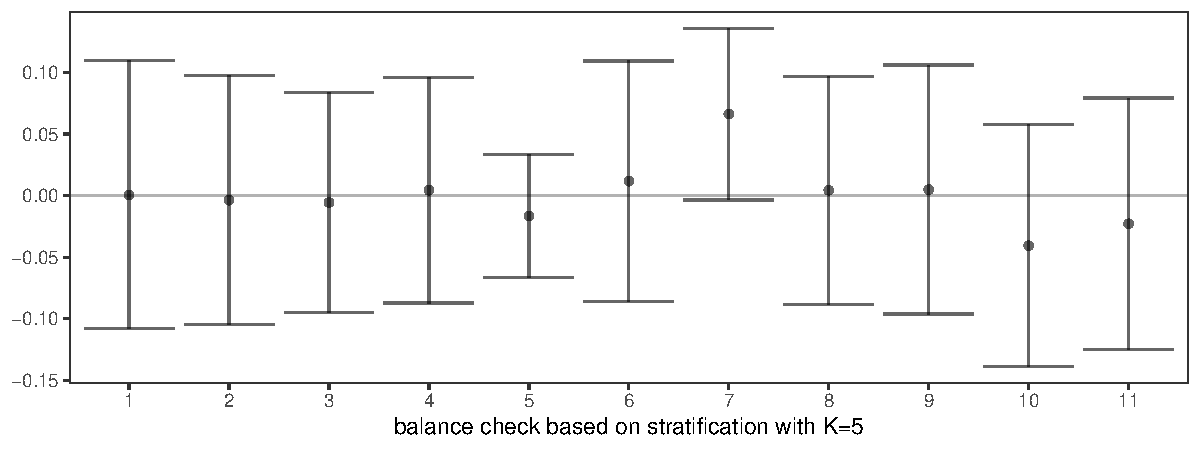
\includegraphics[width = \textwidth]{figures/balance_PSstratification5.pdf}
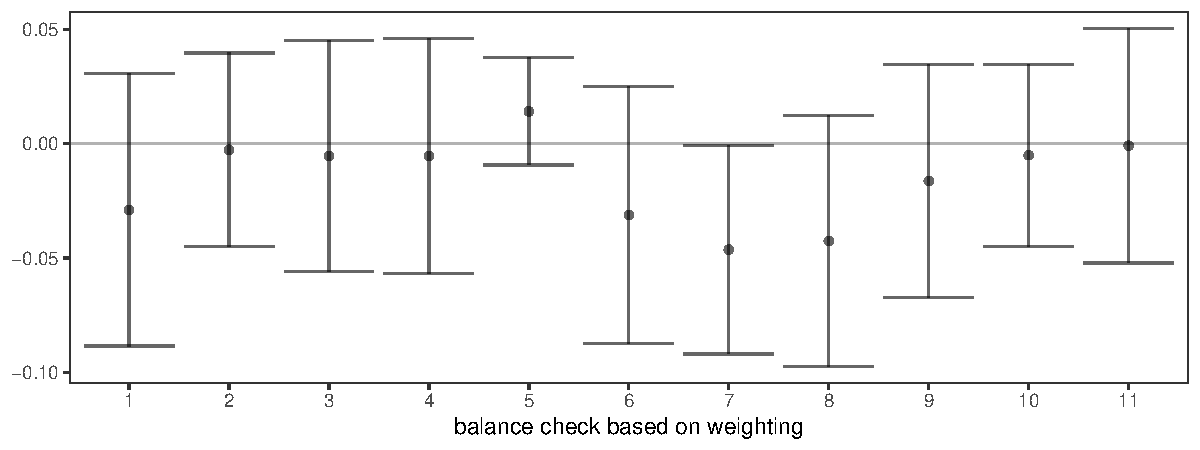
\includegraphics[width = \textwidth]{figures/balance_PShajek.pdf}
\caption{Balance check: point estimates and 95\% confidence intervals of the average causal effect on covariates}\label{fig::balance-check}
\end{figure}

 

 

 
 
 \section{Homework Problems}
 
 
 
 
 \paragraph{Another version of Theorem \ref{thm::pscore-dimreduction}} \label{hw::principal-unobserved-cov}
 Prove that 
\begin{equation}
\label{eq::principal-covariate-ind}
 Z\ind \{  Y(1), Y(0) , X\}  \mid e(X, Y(1), Y(0)   ) .
\end{equation}  
 
 Remark:
 This result holds without assuming strong ignorability. It implies that
 $$
  Z\ind \{  Y(1), Y(0) \}  \mid  \{ X,   e(X, Y(1), Y(0)  \} .
 $$
\citet{rosenbaum2020modern} and \citet{rosenbaum2023propensity} pointed out the result in \eqref{eq::principal-covariate-ind} and called $e(X, Y(1), Y(0)   ) $ the  {\it  principal unobserved covariate}. 
 
 
 
\paragraph{Another version of Theorem \ref{thm::pscore-dimreduction}} 

Theorem \ref{thm::pscore-dimreduction} states a result under strong ignorability. An analogous result also holds under ignorability. 
That is, if ignorability holds conditional on covariates $X$, then it also holds conditional on the scalar propensity score $e(X)$. 

\begin{theorem}
\label{thm::pscore-dimension-reduction-weak-ig}
If $Z\ind Y(z)  \mid X$ for $z=0,1$, then
$
Z\ind Y(z)\mid e(X)
$
for $z=0,1$. 
\end{theorem} 


Prove Theorem \ref{thm::pscore-dimension-reduction-weak-ig}.



 
 \paragraph{More results on the IPW estimators}
\label{hw::hajek-weights} 
 
This is related to the discussion of the HT estimator in Section \ref{sec::ipw-estimators}. First, prove Proposition \ref{prop::no-invariance-HT}.  
Second, prove 
 \begin{eqnarray*} 
E\left\{ \frac{1}{n} \sumn \frac{Z_i }{e(X_i) } \right\} =1,\quad
E\left\{  \frac{1}{n} \sumn \frac{ (1-Z_i) }{ 1 - e(X_i) }  \right\} = 1.
\end{eqnarray*}
Third, prove that if we add a constant $c$ to every observed outcome $Y_i$, the Hajek estimator
$
\hat{\tau}^\textup{hajek} 
$
remains the same. 


\paragraph{Re-analysis of \citet{Rosenbaum::1983JRSSB}}



Table \ref{table::rr1983table1} is from \citet{Rosenbaum::1983JRSSB}, which concerned the causal effect of the coronary artery bypass surgery compared with the medical therapy on the functional improvement 6 months after cardiac catheterization.  They first estimated the propensity score based on 74 observed covariates and then formed 5 strata based on the discretized estimated propensity score. Because the treatment is binary and the outcome is also binary, they represented the data in a table. 
Based on Table \ref{table::rr1983table1} , estimate the average causal effect, and report the 95\% confidence interval of the average causal effect. 



\begin{table}
\caption{Table 1 of \citet{Rosenbaum::1983JRSSB}}\label{table::rr1983table1}
\begin{tabular}{clcc}
\hline 
stratum by $\hat{e}(X)$ & treatment &  number of patients & proportion improved\\
\hline 1 & Surgical & 26 & 0.54 \\
& Medical & 277 & 0.35 \\
2 & Surgical & 68 & 0.70 \\
& Medical & 235 & 0.40 \\
3 & Surgical & 98 & 0.70 \\
& Medical & 205 & 0.35 \\
4 & Surgical & 164 & 0.71 \\
& Medical & 139 & 0.30 \\
5 & Surgical & 234 & 0.70 \\
& Medical & 69 & 0.39 \\
\hline
\end{tabular}
\end{table}


Remark:   If you are interested, you can read the whole paper of \citet{Rosenbaum::1983JRSSB} after reading Part \ref{part::challenges-os} of the book. It is a canonical paper on sensitivity analysis in causal inference. 

 


\paragraph{Balancing score and propensity score: more theoretical results}
\label{hw::balancingscore-rr1983}


\citet{rosenbaum1983central} also introduced the notion of {\it balancing score}.

\begin{definition}
[balancing score]\label{def::balancing-score}
  $b(X)$ is a balancing score if 
  $$
  Z\ind X\mid b(X).
  $$
\end{definition}

In Definition \ref{def::balancing-score},  $b(X)$ can be a scalar or a vector. An obvious balancing score is $b(X) = X$, but it is not a useful one without any simplification of the original covariates. By Theorem \ref{thm::pscoreASbscore}, the propensity score is a special balancing score. More interestingly, \citet{rosenbaum1983central} showed that the propensity score is the coarsest balancing score, as in Theorem \ref{thm::balancingscore} below which includes Theorem \ref{thm::pscoreASbscore} as a special case. 


\begin{theorem}
\label{thm::balancingscore}
$b(X)$ is a balancing score if and only if $b(X)$ is finer than $e(X)$ in the sense that $e(X) = f(b(X))$ for some function $f(\cdot)$. 
\end{theorem}


Theorem \ref{thm::balancingscore} is relevant in subgroup analysis. In particular, we may be interested in not only the average causal effect $\tau$ but also the subgroup effects. For instance, we may want to estimate the average causal effects among boys and girls, respectively. Without loss of generality, assume the first component of $X$ is the indicator for girls, and we are interested in estimating 
$$
\tau(x_1) = E\{ Y(1) - Y(0) \mid X_1 = x_1  \},\quad (x_1=1,0).
$$
Theorem \ref{thm::balancingscore} implies that under ignorability, we also have 
\begin{equation}
\label{eq::subgroup-ignorability}
Z\ind \{ Y(1) , Y(0) \} \mid e(X), X_1
\end{equation}
because $b(X) = \{e(X), X_1\}$ is finer than $e(X)$ and thus a balancing score. The conditional independence in \eqref{eq::subgroup-ignorability} ensures ignorability holds given the propensity score, within each level of $X_1$. Therefore, we can perform the same analysis based on the propensity score, within each level of $X_1$, yielding estimates for two subgroup effects. 


With the above motivation in mind, now prove Theorem \ref{thm::balancingscore}. 


\paragraph{Some basics of subgroup effects}

This problem is related to Problem \ref{hw::balancingscore-rr1983}, but you can work on it independently. 

Consider a standard observational study with covariates $X = (X_1, X_2)$, where $X_1$ denotes a binary subgroup indicator (e.g., statistics major or not statistics major) and $X_2$ contains the rest of the covariates. The parameter of interest is the subgroup causal effect 
$$
\tau(x_1) = E\{ Y(1) - Y(0) \mid X_1 = x_1  \},\quad (x_1=1,0).
$$
Show that
$$
\tau(x_1) =  E\left\{   \frac{  1(X_1 = x_1) ZY}{ e(X) }   - \frac{  1(X_1 = x_1) (1-Z)Y}{ 1 -  e(X) }    \right\} \Big /  \pr(X_1 = x_1)
$$
and give the corresponding HT and Hajek estimators for $\tau(x_1) $. 



 \paragraph{Recommended reading}
 
 
The title of this chapter is the same as the title of the classic paper by \citet{rosenbaum1983central}. Most results in this chapter are directly drawn from their original paper.  


\citet{rubin2007design} and \citet{rubin2008objective} highlighted the importance of the design stage of observational studies for more objective causal inference 
 
